\documentclass[12pt,a4paper,titlepage]{article}
\title{Implementazione dell'algoritmo di One-Sided Jacobi Rotation per la decomposizione SVD, tramite librerie NVIDIA CUDA C (codice C) su piattaforma embedded Jetson TK1 (GPU).} 
\author{Matteo Orlandini \& Jacopo Pagliuca}
\date{}

\usepackage[english, italian ]{babel} %the last declared language is the one used in the document
\usepackage[utf8]{inputenc}
\usepackage[T1]{fontenc}
\usepackage{amsmath}
\usepackage{amssymb}
\usepackage{graphicx}
\usepackage{listings}
%inizio impostazioni bibliografia
\usepackage[autostyle,italian=guillemets]{csquotes} 
%autostyle adatta lo stile delle citazioni alla lingua corrente del documento;
%italian=guillemets racchiude automaticamente tra virgolette caporali
%i campi che prevedono le virgolette;
\usepackage[backend=biber, style=numeric, citestyle=numeric,maxcitenames=99,maxbibnames = 99]{biblatex}
%backend=biber dice a biblatex che s’intende usare Biber come motore bibliografico
%style:numeric Anno di pubblicazione: in fondo al riferimento.
%citestyle=numeric Riferimento: numerico ([1], [2], eccetera).
%fine impostazioni bibliografia

\usepackage{float}
\usepackage{hyperref}
\hypersetup{
	bookmarks=true,         % show bookmarks bar?
	unicode=false,          % non-Latin characters in Acrobat’s bookmarks
	pdftoolbar=true,        % show Acrobat’s toolbar?
	pdfmenubar=true,        % show Acrobat’s menu?
	pdffitwindow=false,     % window fit to page when opened
	pdfstartview={FitH},    % fits the width of the page to the window
	%pdftitle={Relazione di Reti di Sensori Wireless per IOT},    % title
	pdfauthor={Matteo Orlandini},     % author
	pdfsubject={Implementazione dell'algoritmo di One-Sided Jacobi Rotation per la decomposizione SVD, tramite librerie NVIDIA CUDA C (codice C) su piattaforma embedded Jetson TK1 (GPU)},   % subject of the document
	pdfcreator={Matteo Orlandini},   % creator of the document
	%pdfproducer={Producer}, % producer of the document
	pdfpagemode={UseOutlines},
	%bookmarksopen,
	pdfstartview={FitH},
	colorlinks=false,       % false: boxed links; true: colored links
	linkcolor={red},
	citecolor={green},
	urlcolor={cyan}
} 

\usepackage[dvipsnames]{xcolor}
\usepackage{listings}
%http://latexcolor.com/
\definecolor{ivory}{rgb}{1.0, 1.0, 0.94}
\definecolor{lightgoldenrodyellow}{rgb}{0.98, 0.98, 0.82}

\lstset{% general command to set parameter(s)
	backgroundcolor=\color{ivory},
	%backgroundcolor=\color{White}, % choose the background color; you must add \usepackage{color} or \usepackage{xcolor}
	basicstyle=\small,        % the size of the fonts that are used for the code
	breakatwhitespace=false,         % sets if automatic breaks should only happen at whitespace
	breaklines=true,
	captionpos=b,                    % sets the caption-position to bottom
	%extendedchars=true,              % lets you use non-ASCII characters; for 8-bits encodings only, does not work with UTF-8
	keywordstyle=\color{Blue}\bfseries, 	% blue keywords
	language=C,
	classoffset=0,
	morekeywords={bool,ifdef,ifndef,endif},
	keywordstyle=\color{Blue}\bfseries,
	%classoffset=1,
	%morekeywords={},
	%keywordstyle=\color{black}\bfseries,
	classoffset=0,
	identifierstyle=,           % nothing happens
	commentstyle=\color{ForestGreen}, % green comments
	stringstyle=\color{red},  %\ttfamily    % typewriter type for strings
	showstringspaces=false,	% no special string spaces
	numberbychapter=true,
	tabsize=2,
	columns=flexile,
	keepspaces=flase,                 % keeps spaces in text, useful for keeping indentation of code (possibly needs columns=flexible)
	frame=lines,
	literate=
	{á}{{\'a}}1 {é}{{\'e}}1 {í}{{\'i}}1 {ó}{{\'o}}1 {ú}{{\'u}}1
	{Á}{{\'A}}1 {É}{{\'E}}1 {Í}{{\'I}}1 {Ó}{{\'O}}1 {Ú}{{\'U}}1
	{à}{{\`a}}1 {è}{{\`e}}1 {ì}{{\`i}}1 {ò}{{\`o}}1 {ù}{{\`u}}1
	{À}{{\`A}}1 {È}{{\'E}}1 {Ì}{{\`I}}1 {Ò}{{\`O}}1 {Ù}{{\`U}}1
	{ä}{{\"a}}1 {ë}{{\"e}}1 {ï}{{\"i}}1 {ö}{{\"o}}1 {ü}{{\"u}}1
	{Ä}{{\"A}}1 {Ë}{{\"E}}1 {Ï}{{\"I}}1 {Ö}{{\"O}}1 {Ü}{{\"U}}1
	{â}{{\^a}}1 {ê}{{\^e}}1 {î}{{\^i}}1 {ô}{{\^o}}1 {û}{{\^u}}1
	{Â}{{\^A}}1 {Ê}{{\^E}}1 {Î}{{\^I}}1 {Ô}{{\^O}}1 {Û}{{\^U}}1
	{Ã}{{\~A}}1 {ã}{{\~a}}1 {Õ}{{\~O}}1 {õ}{{\~o}}1
	{œ}{{\oe}}1 {Œ}{{\OE}}1 {æ}{{\ae}}1 {Æ}{{\AE}}1 {ß}{{\ss}}1
	{ű}{{\H{u}}}1 {Ű}{{\H{U}}}1 {ő}{{\H{o}}}1 {Ő}{{\H{O}}}1
	{ç}{{\c c}}1 {Ç}{{\c C}}1 {ø}{{\o}}1 {å}{{\r a}}1 {Å}{{\r A}}1
	{€}{{\euro}}1 {£}{{\pounds}}1 {«}{{\guillemotleft}}1
	{»}{{\guillemotright}}1 {ñ}{{\~n}}1 {Ñ}{{\~N}}1 {¿}{{?`}}1
}    

\addbibresource{Bibliografia.bib}

\begin{document}

\begin{titlepage}
	
	\centering
	
\includegraphics[width=.2\textwidth]{Immagini/univpmlogo}\par\vspace{1cm}
	{\scshape\LARGE Università Politecnica delle Marche\par}
	\vspace{1cm}
	{\scshape\Large Sistemi Embedded\par}
	\vspace{1.5cm}
	{\huge\bfseries Implementazione dell'algoritmo di One-Sided Jacobi Rotation per la decomposizione SVD, tramite librerie NVIDIA CUDA C (codice C) su piattaforma embedded Jetson TK1 (GPU). \par}
	\vspace{2cm}
	{\Large\itshape Matteo Orlandini \par}
	{\Large\itshape Jacopo Pagliuca\par}
	\vfill
	supervisionato da\par
	Dott. Laura \textsc{Falaschetti} e Prof. Claudio \textsc{Turchetti}
	
	\vfill
	
	% Bottom of the page
	{\large \today\par}
\end{titlepage}

\tableofcontents

\section{Introduzione}
\label{sec:Introduzione}
La seguente tesina descrive il lavoro svolto per la progettazione di un algoritmo di One-sided Jacobi per la decomposizione in valori singolari (SVD) di una matrice, tramite librerie NVIDIA CUDA C. Il codice è stato testato e pensato per una piattaforma embedded Jetson TK1.

La Jetson TK1 è una scheda grafica embedded realizzato dalla NVIDIA che contiene un processore Tegra K1 SoC nella variante T124. Inoltre essa possiede un sistema operativo Ubuntu Linux ed ha installata la versione di CUDA 6.5. La compute capability della GPU, cioè la capacità di calcolo che determina le specifiche generali e le funzionalità disponibili, è pari a 3.2.

In facoltà era già stato sviluppato un codice in C per la SVD ottimizzato per lavorare su CPU. Il nostro lavoro era quello di confrontare i nostri risultati con quelli precedentemente ottenuti e valutare la possibilità di una implementazione alternativa che sfruttasse appieno le potenzialità del calcolo parallelo della GPU della Jetson.

Come base per il nostro lavoro abbiamo studiato il linguaggio di programmazione e l’architettura CUDA in~\cite{Cheng:ProfessionalCudaProgramming} e~\cite{Sanders:CudaByExample}. In seguito sono stati analizzati gli articoli~\cite{Acosta:SVD},~\cite{Boukaram:SVD},~\cite{Lahabar:SVD} e~\cite{Romer:SVD} che descrivevano vari approcci per l’ottimizzazione dell’algoritmo su GPU, per poi realizzare la nostra versione, i cui risultati sono molto simili a quelli ottenuti negli articoli. 

Per lavorare sulla scheda abbiamo sfruttato il protocollo SSH dal dipartimento, in modo da connettersi alla scheda da remoto. Alla fine della realizzazione del progetto non è però stato possibile accedere al dipartimento e quindi riportare i risultati esatti del tempo computazionale che necessita l’algoritmo sulla Jetson. Abbiamo quindi usato come riferimento una NVIDIA GTX 610M, i cui risultati sono proporzionali a quelli ottenuti con la
Jetson.

\subsection{SVD}
In algebra lineare, la decomposizione ai valori singolari (SVD), è una fattorizzazione di una matrice in tre diverse matrici basata sull'uso di autovalori e autovettori.

La decomposizione di una matrice $\mathbf{A}$ si basa sul \textit{teorema fondamentale dell'algebra lineare}: 

Data una matrice $\mathbf{A}\in\mathbb{C}^{m\times n}$ di rango $\rho$, la decomposizione in valori singolari di $\mathbf{A}$ è rappresentata dal prodotto di due matrici unitarie $\mathbf{U}\in\mathbb{C}^{m\times m}$, $\mathbf{V}\in\mathbb{C}^{n\times n}$ e una matrice diagonale $\mathbf{\Sigma}\in\mathbb{R}^{m\times n}$, come mostrato in (\ref{svd}).
\begin{equation}\label{svd}
\mathbf{A}=\mathbf{U}\mathbf{\Sigma}\mathbf{V}^H
\end{equation}
Le colonne di $\mathbf{U}$ sono chiamate \textit{vettori singolari sinistri} di $\mathbf{A}$ mentre le colonne di $\mathbf{V}$ sono i \textit{vettori singolari destri} di $\mathbf{A}$. Inoltre, $\mathbf{\Sigma}$ è una matrice reale non negativa del tipo
\[
\Sigma=\begin{bmatrix}
\sigma_1 & 0 & 0 & 0\\
0 & \ddots & 0 & 0\\
0 & 0 & \sigma_{\rho} & 0\\
0 & 0 & 0 & 0
\end{bmatrix}
\]
Gli elementi diagonali di $\Sigma$ sono i \textit{valori singolari} di $\mathbf{A}$ e sono solitamente in ordine decrescente: $\sigma_1 \geq \sigma_2 \geq ... \geq \sigma_{\rho} > 0, \sigma_{\rho+1}=...=0$.

Nel caso in cui $\mathbf{A}\in\mathbb{R}^{m\times n}$ l'equazione (\ref{svd}) diventa:
\begin{equation}\label{svd2}
\mathbf{A}=\mathbf{U}\mathbf{\Sigma}\mathbf{V}^T
\end{equation}
dove $\mathbf{U}\in\mathbb{R}^{m\times m}$ e $\mathbf{V}\in\mathbb{R}^{n\times n}$ sono matrici ortonormali.
\begin{eqnarray}
\mathbf{U}\mathbf{U}^T=\mathbf{U}^T\mathbf{U}=I^{m\times m}\\
\mathbf{V}\mathbf{V}^T=\mathbf{V}^T\mathbf{V}=I^{n\times n}
\end{eqnarray}
Unendo queste due proprietà all'equazione (\ref{svd2}) si possono ricavare l'espressione di $\mathbf{A}\mathbf{A}^T$:
\[
\mathbf{A}\mathbf{A}^T=\mathbf{U}\mathbf{\Sigma}\mathbf{V}^T(\mathbf{U}\mathbf{\Sigma}\mathbf{V}^T)^T=\mathbf{U}\mathbf{\Sigma}\mathbf{V}^T\mathbf{V}\mathbf{\Sigma}\mathbf{U}^T=\mathbf{U}\mathbf{\Sigma}^2\mathbf{U}^T
\]
Allo stesso modo, per $\mathbf{A}^T\mathbf{A}$:
\[
\mathbf{A}^T\mathbf{A}=\mathbf{V}\mathbf{\Sigma}^2\mathbf{V}^T
\]
La SVD ha numerose applicazioni nel campo dell'algebra lineare. Innanzitutto fornisce delle informazioni importanti sulla matrice $\mathbf{A}$, come il suo rango, qual è il suo nucleo e qual è la sua immagine. Viene usata per definire la pseudo-inversa di una matrice rettangolare utile per la risoluzione del problema dei minimi quadrati. Trova utilizzo anche nella risoluzione di sistema di equazioni lineari omogeneo.

Un'altra importante applicazione riguarda l'approssimazione della matrice $\mathbf{A}$, con una di rango inferiore (SVD troncata), utilizzata nell'elaborazione di immagini e nell'elaborazione dei segnali.

La SVD ha anche note applicazioni nel campo dell'analisi delle componenti principali.




\subsection{One Sided Jacobi SVD}
\label{sec:OneSidedJacobi}
\label{sec:OneSidedJacobi}
Per effettuare la SVD di una matrice, sono stati sviluppati numerosi algoritmi con lo scopo di ottimizzare il numero di operazioni svolte dalla macchina.
Uno di quelli più usati è l'algoritmo di Jacobi con la sua variante One Sided Jacobi. L'approccio utilizzato è quello di applicare successive rotazioni alla matrice originale, in modo da azzerare le componenti che si trovino al di fuori della diagonale. Tramite diverse iterazioni, si ottiene come risultato finale una matrice diagonale contenente i valori singolari richiesti.
\subsubsection{Jacobi rotation}
\label{sec:Jacobi_rotation}
La rotazione di Jacobi è una operazione che consente di azzerare selettivamente elementi specifici di una matrice. Tramite una rotazione in due dimensioni $p$ e $q$ vengono azzerati gli elementi $(p,q)$ e $(q,p)$ della matrice.

L'operazione si basa sull'utilizzo della matrice di Jacobi $\mathbf{J}(p,q,\theta)$ del tipo:
\begin{equation}
\mathbf{J}(p,q,\theta)=\begin{bmatrix}
1 &  &  &  &  &  & \\
& \ddots &  &  &  & 0 & \\
&  & c & \cdots & -s &  & \\
&  & \vdots & \ddots & \vdots &  & \\
&  & s & \cdots & c &  & \\
& 0 &  &  &  & \ddots & \\
&  &  &  &  &  & 1
\end{bmatrix}
\end{equation}
dove $c=\cos(\theta)$ e $s=\sin(\theta)$, vengono applicati solo nelle dimensioni $p$ e $q$.

Premoltiplicare un vettore per $\mathbf{J}(p,q,\theta)^T$ equivale a ruotarlo in senso antiorario di un angolo $\theta$ nel piano $(p,q)$. Questa rotazione produce un vettore risultante nel quale la componente q è stata azzerata. Infatti se $\mathbf{x}\in\mathbb{R}^{n}$ e
\begin{equation}
\mathbf{y}=\mathbf{J}(p,q,\theta)^T	\cdot \mathbf{x}
\end{equation}
allora
\begin{eqnarray}
y_p=cx_p-sx_q\\
y_q=sx_p+cx_q\label{yq}\\
y_i=x_i, ~ i\neq p,q
\end{eqnarray}
Da \eqref{yq} si nota che $y_q$ può essere azzerata ponendo:
\begin{equation}
c=\frac{x_p}{\sqrt{x_p^2+x_q^2}},\quad s=\frac{-x_q}{\sqrt{x_p^2+x_q^2}}
\end{equation}
Per una matrice $\mathbf{A}$ simmetrica, è possibile azzerare le componenti $(p,q)$ e $(q,p)$ applicando la\eqref{jacrot}.
\begin{equation}\label{jacrot}
\mathbf{B}=\mathbf{J}(p,q,\theta)^T\mathbf{A}\mathbf{J}(p,q,\theta)
\end{equation}

\subsubsection{Algoritmo One Sided Jacobi}
\label{sec:Algoritmo_One_Sided_Jacobi}
L'idea base per questo algoritmo è quella di ruotare le colonne i e j di $\mathbf{A}$ per renderle ortogonali. In questo modo, le colonne i e j di $\mathbf{A}^T\mathbf{A}$ saranno implicitamente ortogonali.

Sia $\mathbf{J}(p,q,\theta)$ la matrice di rotazione che, applicata ad $\mathbf{A}$, produce:
\begin{equation}
\mathbf{B}=\mathbf{AJ}
\end{equation}
dove le colonne i e j di $\mathbf{B}$ sono date da
\begin{eqnarray}
b_{:i}=ca_{:i}-sa_{:j}\\
b_{:j}=sa_{:i}+ca_{:j}
\end{eqnarray}
l'elemento $(B^TB)_{ij}$ sarà
\[
(B^TB)_{ij}=b_{:i}^Tb_{:j}=(ca_{:i}-sa_{:j})^T(sa_{:i}+ca_{:j})
\]
assumendo $(B^TB)_{ij}=0,i\neq j$ si ottiene
\[
cs(||a_{:i}||^2-||a_{:j}||^2)+(c^2-s^2)(sa_{:i}+ca_{:j})
\]
Dividendo per $c^2$ e considerando
\begin{equation*}
\begin{aligned}
t=s/c\\
\alpha = ||a_{:i}||^2\\
\beta = ||a_{:j}||^2\\
\gamma = a_{:i}^Ta_{:j}\\
\tau =(\beta - \alpha)/2\gamma
\end{aligned}
\end{equation*}
si ottiene la seguente espressione:
\begin{equation}
t^2+2\tau t-1=0
\end{equation}
Risolvendo e scegliendo come soluzione la radice con il minore valore assoluto,
\begin{equation}
t=min|-\tau\pm\sqrt{1+\tau^2}|
\end{equation}
ottieniamo i valori di c e s che rappresentano coseno e seno nella matrice di rotazione:
\begin{equation}
c=\frac{1}{\sqrt{1+t^2}},\quad s=ct
\end{equation}
Con c e s così calcolati, gli elementi $(B^TB)_{ij}$ e $(B^TB)_{ji}$ saranno uguali a zero.\cite{Turchetti:SVDAlgorithms}





\subsection{CUDA}
%CUDA: spiegazione del funzionamento della GPU 
%\fullcite{Cheng:ProfessionalCudaProgramming}
\subsection{Calcolo parallelo}
Negli ultimi decenni, c'è stato un crescente interesse per il calcolo parallelo. L'obiettivo primario del calcolo parallelo è migliorare la velocità di calcolo.

Il calcolo parallelo può essere definito come una forma di calcolo in cui molte operazioni vengono eseguitie simultaneamente, in base al principio che spesso i problemi di grandi dimensioni possono essere suddivisi in problemi più piccoli, che vengono poi risolti contemporaneamente.

Dal punto di vista del programmatore, una domanda naturale è come mappare i calcoli simultanei sui computer. Supponendo di avere più risorse informatiche, il calcolo parallelo può quindi essere definito come l'uso simultaneo di più risorse di calcolo (core o computer) per eseguire i calcoli simultanei. Un grosso problema viene suddiviso in problemi più piccoli, ciascuno dei quali viene quindi risolto contemporaneamente su diverse risorse di elaborazione. Gli aspetti software e hardware del calcolo parallelo sono strettamente intrecciati insieme. In effetti, il calcolo parallelo di solito coinvolge due aree distinte delle tecnologie informatiche:
\begin{itemize}
	\item Computer architecture (aspetto hardware)
	\item Parallel programming (aspetto software)
\end{itemize}
La computer architecture si concentra sul supporto del parallelismo a livello architettonico, mentre il parallel programming si concentra sulla risoluzione di un problema simultaneamente sfruttando appieno il potere computazionale dell'architettura del computer. Per ottenere l'esecuzione parallela nel software, l'hardware deve fornire una piattaforma che supporti l'esecuzione simultanea di più processi o thread multipli.

I processori più moderni implementano l'\emph{architettura Harvard}, come mostrato in Figura~\ref{fig:Harvard_architecture}, che comprende tre componenti principali:
\begin{itemize}
	\item Memoria (instruction memory e data memory)
	\item Central processing unit (control unit e arithmetic logic unit)
	\item Interfacce di Input/Output
\end{itemize}
\begin{figure}[h!]
	\centering
	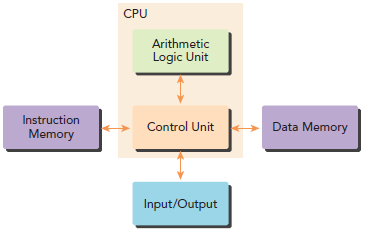
\includegraphics[width=.5\textwidth]{Immagini/CUDA/Harvard_architecture}
	\caption{Architettura Harvard \cite{Cheng:ProfessionalCudaProgramming}}
	\label{fig:Harvard_architecture}
\end{figure}
La componente chiave nell'elaborazione è la CPU, generalmente chiamata core. Al giorno d'oggi, la tendenza nella progettazione dei chip è quella di integrare più core in un singolo processore, generalmente definito multicore, per supportare il parallelismo a livello di architettura. Pertanto, la programmazione può essere vista come il processo di mappatura del calcolo di un problema ai core disponibili in modo tale da ottenere l'esecuzione parallela.

Quando si implementa un algoritmo sequenziale, potrebbe non essere necessario comprendere i dettagli dell'architettura del computer per scrivere un programma corretto. Tuttavia, quando si implementano algoritmi per macchine multicore, è molto più importante che i programmatori siano consapevoli delle caratteristiche dell'architettura del computer sottostante. La scrittura di programmi paralleli sia corretti che efficienti richiede una conoscenza fondamentale delle architetture multicore.
\subsection{Calcolo sequenziale e parallelo}
Quando si scrive un programma, è naturale dividere il problema in una serie discreta di calcoli; ogni calcolo esegue un'attività specifica, come mostrato in Figura~\ref{fig:Execution_order_sequential}. Questo tipo di programma è chiamato \emph{sequenziale}.
\begin{figure}[h!]
	\centering
	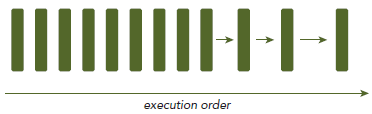
\includegraphics[width=.5\textwidth]{Immagini/CUDA/Execution_order_sequential}
	\caption{Ordine di esecuzione sequenziale \cite{Cheng:ProfessionalCudaProgramming}}
	\label{fig:Execution_order_sequential}
\end{figure}
Esistono due modi per classificare la relazione tra due pezzi di codice: alcuni sono
correlati da un vincolo di precedenza e pertanto devono essere calcolati in sequenza; altri non hanno tali restrizioni e possono essere calcolati contemporaneamente. Qualsiasi programma contenente attività eseguite contemporaneamente è chiamato \emph{parallelo}. Come mostrato in Figura~\ref{fig:Execution_order_parallel}, un programma parallelo può avere alcune parti sequenziali.
\begin{figure}[H]
	\centering
	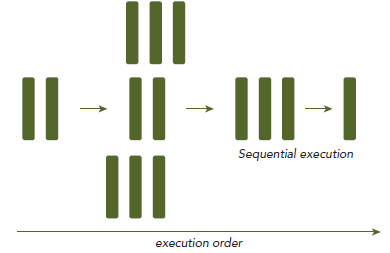
\includegraphics[width=.5\textwidth]{Immagini/CUDA/Execution_order_parallel}
	\caption{Ordine di esecuzione parallelo \cite{Cheng:ProfessionalCudaProgramming}}
	\label{fig:Execution_order_parallel}
\end{figure}
\subsection{Struttura di programmazione CUDA}
Il modello di programmazione CUDA consente di eseguire applicazioni su sistemi di elaborazione eterogenei semplicemente annotando il codice con una piccola serie di estensioni al linguaggio di programmazione C. Un ambiente eterogeneo è costituito da CPU integrate da GPU, ognuna con la propria memoria separata da un bus PCI-Express. Pertanto, è necessario notare la seguente distinzione:
\begin{itemize}
	\item \textbf{Host}: la CPU e la sua memoria (host memory)
	\item \textbf{Device}: la GPU e la sua memoria (device memory)
\end{itemize}
Un componente chiave del modello di programmazione CUDA è il kernel, cioè il codice che viene eseguito sul device GPU. CUDA gestisce i kernel scritti dai programmatori su thread GPU. Dall'host, si definisce il modo in cui l'algoritmo viene mappato sul device in base ai dati dell'applicazione e alla capacità del device GPU. 

L'host può funzionare indipendentemente dal dispositivo per la maggior parte delle operazioni. Quando si chiama un kernel, il controllo viene immediatamente restituito all'host, liberando la CPU per eseguire task aggiuntivi. Un tipico programma CUDA è costituito da un codice seriale integrato da un codice parallelo. Come mostrato in Figura~\ref{fig:Cuda_programming_structure}, il codice seriale (così come quello parallelo) viene eseguito sull'host, mentre il codice parallelo viene eseguito sul device. Il codice del device è scritto usando CUDA C. È possibile inserire tutto il codice in un singolo file sorgente oppure utilizzare più file sorgente per creare l'applicazione o le librerie. Il compilatore NVIDIA C (nvcc) genera il codice eseguibile sia per l'host che per il device.
\begin{figure}[H]
	\centering
	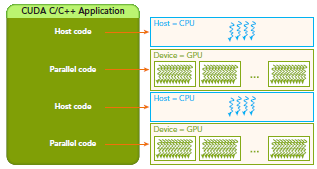
\includegraphics[width=.75\textwidth]{Immagini/CUDA/Cuda_programming_structure}
	\caption{Struttura di programmazione Cuda \cite{Cheng:ProfessionalCudaProgramming}}
	\label{fig:Cuda_programming_structure}
\end{figure}

Un flusso di elaborazione tipico di un programma CUDA segue questo modello:
\begin{enumerate}
	\item Copia i dati dalla memoria della CPU alla memoria della GPU.
	\item Chiama i kernel per operare sui dati memorizzati nella memoria della GPU.
	\item Copia i dati dalla memoria della GPU alla memoria della CPU.
\end{enumerate}
\subsection{Organizzazione della memoria}
\label{sec:managing_memory}
Il modello di programmazione CUDA presuppone un sistema composto da un host e un device, ognuno con una propria memoria separata. I kernel funzionano con la memoria del device. Per consentire il pieno controllo e ottenere le migliori prestazioni, CUDA fornisce funzioni per allocare la memoria del dispositivo, liberare la memoria del dispositivo e trasferire i dati tra la memoria host e quella device. La Tabella~\ref{table:Host and Device Memory Functions} elenca le funzioni C standard e le corrispondenti funzioni CUDA C per le operazioni sulla memoria.
\begin{table}[h!]
	\centering
	\begin{tabular}{c c} 
		\hline
		FUNZIONI C STANDARD & FUNZIONI CUDA C\\
		\hline
		malloc & cudaMalloc\\
		\hline
		memcpy & cudaMemcpy\\
		\hline
		memset & cudaMemset\\
		\hline
		free & cudaFree\\
		\hline
	\end{tabular}
	\caption{Funzioni sulla memoria host e device}
	\label{table:Host and Device Memory Functions}
\end{table}
La funzione utilizzata per eseguire l'allocazione della memoria GPU è cudaMalloc e la sua struttura è:
\begin{lstlisting}[label=code:cudaMalloc_def]
cudaError_t cudaMalloc ( void** devPtr, size_t size )
\end{lstlisting}
Questa funzione alloca un intervallo lineare di memoria del dispositivo con la \emph{size} specificata in byte. La memoria allocata viene restituita tramite \emph{devPtr}. La somiglianza tra cudaMalloc e la libreria runtime standard malloc è intenzionale e ha lo scopo di mantenere l'interfaccia il più vicino possibile alle librerie di runtime C standard.

La funzione utilizzata per trasferire i dati tra l'host e il device è: cudaMemcpy e la sua struttura è:
\begin{lstlisting}[label=code:cudaMemcpy_def]
cudaError_t cudaMemcpy ( void* dst, const void* src, size_t count, cudaMemcpyKind kind )
\end{lstlisting}
Questa funzione copia i byte specificati dall'area di memoria di origine, indicata da \emph{src}, nell'area di memoria di destinazione, indicata da \emph{dst}, con la direzione specificata dal tipo, dove \emph{kind} assume uno dei seguenti tipi:
\begin{itemize}
	\item cudaMemcpyHostToHost
	\item cudaMemcpyHostToDevice
	\item cudaMemcpyDeviceToHost
	\item cudaMemcpyDeviceToDevice
\end{itemize}
Questa funzione mostra un comportamento sincrono perché l'applicazione host si blocca fino a quando cudaMemcpy ritorna e il trasferimento è completo. Ogni chiamata CUDA, ad eccezione del lancio del kernel, restituisce un codice di errore di tipo enumerato cudaError\_t. Ad esempio, se la memoria GPU è allocata correttamente, restituisce:

\textit{cudaSuccess}\\
Altrimenti, ritorna:

\textit{cudaErrorMemoryAllocation}
È possibile convertire un codice di errore in un messaggio di errore human-readable con la seguente funzione di runtime CUDA:
\begin{lstlisting}[label=code:cudaGetErrorString_def]
char* cudaGetErrorString(cudaError_t error)
\end{lstlisting}

La funzione cudaGetErrorString è analoga alla funzione standard C strerror.
Il modello di programmazione CUDA espone un'astrazione della gerarchia di memoria dall'architettura GPU. La Figura~\ref{fig:GPU_Memory_Structure} illustra una struttura di memoria GPU semplificata, contenente due ingredienti principali: global memory e shared memory. Un approfondimento sulla gerarchia di memoria della GPU è presente nel capitolo~\ref{sec:CUDA Memory Model}.
\begin{figure}[h!]
	\centering
	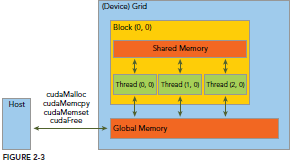
\includegraphics[width=.85\textwidth]{Immagini/CUDA/GPU_Memory_Structure}
	\caption{Struttura della memoria GPU \cite{Cheng:ProfessionalCudaProgramming}}
	\label{fig:GPU_Memory_Structure}
\end{figure}
Una delle caratteristiche più notevoli del modello di programmazione CUDA è la gerarchia di memoria esposta. Ogni dispositivo GPU ha un set di diversi tipi di memoria utilizzati per scopi diversi. Un approfondimento su questa gerarchia è presente nel capitolo~~\ref{sec:CUDA Memory Model}. La global memory è analoga alla memoria di sistema della CPU, mentre la shared memory è simile alla cache della CPU. Tuttavia, lashared memory può essere controllata direttamente da un kernel CUDA C.

\subsection{Organizzazione dei thread}
Quando un kernel viene avviata dal lato host, l'esecuzione viene spostata sul device in cui viene generato un numero elevato di thread e ogni thread esegue le istruzioni specificate dalla funzione kernel. Saper organizzare i thread è una parte fondamentale della programmazione CUDA che espone un'astrazione della gerarchia di thread per consentire di organizzare i thread. Questa è una gerarchia di thread a due livelli composta in blocchi di thread e griglie di blocchi, come mostrato in Figura~\ref{fig:Thread_hierarchy}.
\begin{figure}[h!]
	\centering
	\includegraphics[width=.7\textwidth]{Immagini/CUDA/Thread_hierarchy}
	\caption{Thread hierarchy \cite{Cheng:ProfessionalCudaProgramming}}
	\label{fig:Thread_hierarchy}
\end{figure}
Tutti i thread generati da un singolo lancio del kernel sono collettivamente chiamati griglia. Tutti i thread in una griglia condividono lo stesso spazio di global memory. Una griglia è composta da molti blocchi di thread. Un blocco thread è un gruppo di thread che possono cooperare tra loro usando:
\begin{itemize}
	\item sincronizzazione dei blocchi locali
	\item shared memory dei blocchi locali
\end{itemize}
Threads da blocchi diversi non possono cooperare. I threads si basano sulle seguenti due coordinate univoche per distinguersi l'una dall'altra:
\begin{itemize}
	\item blockIdx (indice del blocco all'interno di una griglia)
	\item threadIdx (indice del thread all'interno di un blocco)
\end{itemize}
Queste variabili appaiono come variabili predefinite pre-inizializzate a cui è possibile accedere nei kernel. Quando viene eseguita un kernel, le variabili di coordinate blockIdx e threadIdx vengono assegnate a ciascun thread dal CUDA runtime. Sulla base delle coordinate, è possibile assegnare porzioni di dati a thread diversi.

La variabile di coordinate è di tipo uint3. È una struttura contenente tre numeri interi senza segno e la prima, seconda e terza componente è accessibile attraverso i campi x, y e z.

blockIdx.x

blockIdx.y

blockIdx.z

threadIdx.x

threadIdx.y

threadIdx.z

CUDA organizza griglie e blocchi in tre dimensioni. La Figura~\ref{fig:Thread_hierarchy} mostra un esempio di una struttura gerarchica di thread con una griglia 2D contenente blocchi 2D. Le dimensioni di una griglia e di un blocco sono specificate dalle seguenti due variabili integrate:
\begin{itemize}
	\item blockDim (dimensione del blocco, misurata in threads)
	\item gridDim (dimensione della griglia, misurata in blocchi)
\end{itemize}
Queste variabili sono di tipo dim3, un tipo di vettore intero basato su uint3 utilizzato per specificare le dimensioni. Quando si definisce una variabile di tipo dim3, qualsiasi componente lasciato non specificato viene inizializzato su 1. Ogni componente in una variabile di tipo dim3 è accessibile attraverso i suoi campi x, y e z, rispettivamente, come mostrato dai campi mostrati di seguito:

blockDim.x

blockDim.y

blockDim.z
\subsection{Modello della memoria CUDA}
\label{sec:CUDA Memory Model}
Per i programmatori, ci sono generalmente due classificazioni di memoria:
\begin{itemize}
	\item Programmabile: si controlla esplicitamente quali dati vengono inseriti nella memoria programmabile.
	\item Non programmabile: non si ha alcun controllo sul posizionamento dei dati e si fa affidamento su tecniche automatiche per ottenere buone prestazioni.
\end{itemize}
Nella gerarchia di memoria della CPU, la cache L1 e la cache L2 sono esempi di memoria non programmabile. CUDA espone molti tipi di memoria programmabile:
\begin{itemize}
	\item Registers
	\item Shared memory
	\item Local memory
	\item Constant memory
	\item Texture memory
	\item Global memory
\end{itemize}
La Figura~\ref{fig:GPU_Memory_Hierarchy} illustra la gerarchia di questi spazi di memoria. Ognuno ha un diverso ambito, durata e comportamento di memorizzazione nella cache.
\begin{figure}[h!]
	\centering
	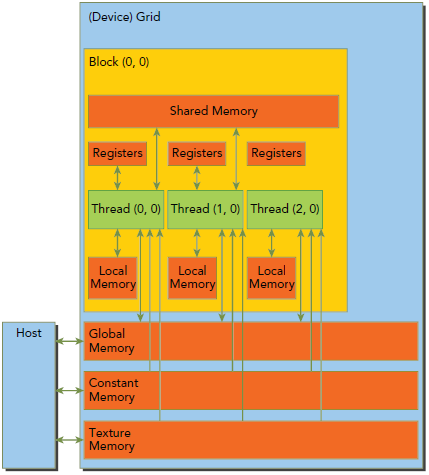
\includegraphics[width=.7\textwidth]{Immagini/CUDA/GPU_Memory_Hierarchy}
	\caption{Gerarchia della memoria della GPU \cite{Cheng:ProfessionalCudaProgramming}}
	\label{fig:GPU_Memory_Hierarchy}
\end{figure}
Un thread in un kernel ha la sua local memory privata. Un blocco di thread ha una propria memoria shared, visibile a tutti i thread nello stesso blocco thread e il cui contenuto persiste per la durata del blocco thread. Tutti i thread possono accedere alla memoria globale. Esistono anche due spazi di memoria di sola lettura accessibili da tutti i thread: la memoria costante e texture. Gli spazi di memoria globale, costante e texture sono ottimizzati per usi diversi. La Texture memory offre diverse modalità di indirizzo. I contenuti della memoria globale, costante e texture hanno la stessa durata di un'applicazione.
\subsubsection{Registri}
I registri sono lo spazio di memoria più veloce su una GPU. Una variabile dichiarata in un kernel senza altri qualificatori di tipo viene generalmente memorizzata in un registro. Le matrici dichiarate in un kernel possono anche essere memorizzate in registri, ma solo se gli indici utilizzati per fare riferimento alla matrice sono costanti e possono essere determinati al momento della compilazione.

Le variabili nei registri sono private per ogni thread. Un kernel in genere usa i registri per contenere variabili thread private a cui si accede frequentemente. Le variabili nei registri condividono la loro durata con il kernel. Una volta che un kernel ha completato l'esecuzione, non è possibile accedere nuovamente a una variabile nel registro.

I registri sono risorse scarse che vengono suddivise tra gli warp attivi nella Shared Memory (SM).

\subsubsection{Local Memory}
Le variabili in un kernel idonee per i registri ma che non possono rientrare nello spazio di registro allocato per quel kernel si riverseranno nella memoria locale. Le variabili che è probabile che il compilatore inserisca nella memoria locale sono:
\begin{itemize}
	\item Array locali referenziate con indici i cui valori non possono essere determinati in fase di compilazione.
	\item Grandi strutture locali o array che consumerebbero troppo spazio sui registri.
	\item Qualsiasi variabile che non rientra nel limite del registro del kernel.
\end{itemize}
Il nome "memoria locale" è fuorviante: i valori riversati nella memoria locale risiedono nella stessa posizione fisica della memoria globale, quindi gli accessi alla memoria locale sono caratterizzati da elevata latenza e bassa larghezza di banda e sono soggetti ai requisiti per un accesso efficiente alla memoria.

\subsubsection{Shared Memory}
Le variabili con il seguente attributo in un kernel sono immagazzinate nella memoria condivisa:

\_\_shared\_\_ \\

Poiché la shared memory è su chip, ha una larghezza di banda molto più elevata e una latenza molto inferiore rispetto alla memoria locale o globale. È usato in modo simile alla cache L1 della CPU, ma è anche programmabile.

Ogni SM ha una quantità limitata di memoria condivisa che è partizionata tra i blocchi di thread. Pertanto, è necessario fare attenzione a non utilizzare eccessivamente la memoria condivisa o si limiterà inavvertitamente il numero di orditi attivi.

La memoria condivisa è dichiarata nell'ambito di una funzione del kernel ma condivide la sua durata con un blocco di thread. Quando viene eseguito il blocco, la sua allocazione di memoria condivisa verrà rilasciata e assegnata ad altri blocchi thread.

La shared memory serve come mezzo di base per la comunicazione tra thread. I thread all'interno di un blocco possono cooperare condividendo i dati memorizzati nella memoria condivisa. L'accesso alla shared memory deve essere sincronizzato utilizzando la seguente chiamata:
\begin{lstlisting}[label=code:syncthreads_def]
void __syncthreads();
\end{lstlisting}
Questa funzione crea una barriera che tutti i thread nello stesso blocco di thread devono raggiungere prima di poter procedere con qualsiasi altro thread. Creando una barriera per tutti i thread all'interno di un blocco, è possibile prevenire un potenziale rischio di dati. Si verificano quando esiste un ordinamento indefinito di accessi multipli nella stessa posizione di memoria da thread diversi, in cui almeno uno di questi accessi è una scrittura. \_syncthreads può anche influire sulle prestazioni costringendo la SM a rimanere inattiva frequentemente.

\subsubsection{Constant Memory}
La memoria costante risiede nella memoria del device ed è memorizzata nella cache costante dedicata per la SM. Una variabile costante ha il seguente attributo:

\_\_constant\_\_ \\

Le variabili costanti devono essere dichiarate globalmente, al di fuori di qualsiasi kernel. È possibile dichiarare una quantità limitata di memoria costante: 64 KB. La memoria costante viene dichiarata staticamente ed è visibile a tutti i kernel.

I kernel possono sololeggere  dalla memoria costante che deve quindi essere inizializzata dall'host utilizzando:
\begin{lstlisting}[label=code:cudaMemcpyToSymbol_def]
cudaError_t cudaMemcpyToSymbol(const void* symbol, const void* src, size_t count);
\end{lstlisting}
Questa funzione copia i byte di conteggio dalla memoria a cui punta \emph{src} alla memoria a cui punta il simbolo, che è una variabile che risiede sul dispositivo nella memoria globale o costante. Questa funzione è sincrona nella maggior parte dei casi.

La memoria costante funziona meglio quando tutti i thread in un warp leggono dallo stesso indirizzo di memoria. Ad esempio, è opportuno scrivere un coefficiente per una formula matematica nella memoria costante perché tutti i thread useranno lo stesso numero per condurre lo stesso calcolo su dati diversi. Se ogni thread in un warp legge da un indirizzo diverso e legge solo una volta, la memoria costante non è la scelta migliore perché una sola lettura dalla memoria costante si trasmette a tutti i thread in un warp.

\subsubsection{Texture Memory}
La memoria texture si trova nella memoria del device ed è memorizzata in una cache di sola lettura per SM. È un tipo di memoria globale a cui si accede tramite una cache di sola lettura dedicata che include il supporto per il filtro hardware, che può eseguire l'interpolazione in virgola mobile. La memoria texture è ottimizzata per spazi 2D, quindi i thread in un warp che la utilizzano per accedere ai dati 2D otterranno le migliori prestazioni. Per alcune applicazioni, questo è l'ideale e offre un vantaggio in termini di prestazioni grazie alla cache e all'hardware di filtro. Tuttavia, per altre applicazioni l'utilizzo della memoria texture può essere più lento della memoria globale.

\subsubsection{Global Memory}
La memoria globale è la memoria più grande, a più alta latenza e più comunemente usata su una GPU. Il nome \emph{global} si riferisce alla sua portata e durata. È possibile accedere al suo stato sul device per tutta la durata dell'applicazione.

Una variabile nella memoria globale può essere dichiarata staticamente o dinamicamente. Si può dichiarare staticamente una variabile globale nel codice del dispositivo usando il seguente qualificatore:
\_\_device\_\_\\

Nel Capitolo~\ref{sec:managing_memory}, si è definito come allocare dinamicamente la memoria globale dall'host utilizzando cudaMalloc e liberata utilizzando cudaFree. I puntatori alla memoria globale vengono quindi passati alle funzioni del kernel come parametri. Le allocazioni di memoria globale esistono per la durata di un'applicazione e sono accessibili a tutti i thread di tutti i kernel. È necessario prestare attenzione quando si accede alla memoria globale da più thread. Poiché non è possibile sincronizzare l'esecuzione di thread tra blocchi di thread, esiste il potenziale rischio che più thread in blocchi diversi modifichino contemporaneamente la stessa posizione nella memoria globale, il che porterà a un comportamento del programma indefinito.

La memoria globale risiede nella memoria del dispositivo ed è accessibile tramite transazioni di memoria a 32, 64 o 128 byte. Queste transazioni devono essere allineate, cioè il primo indirizzo deve essere un multiplo di 32 byte, 64 byte o 128 byte. L'ottimizzazione delle transazioni di memoria è fondamentale per ottenere prestazioni ottimali. Quando un warp esegue una operazione load/store, il numero di transazioni richieste per soddisfare quella richiesta dipende in genere dai seguenti due fattori:
\begin{itemize}
	\item Distribuzione degli indirizzi di memoria tra i thread del warp.
	\item Allineamento degli indirizzi di memoria per transazione.
\end{itemize}
In generale, maggiore è il numero di transazioni necessarie per soddisfare una richiesta di memoria, maggiore è il potenziale di trasferimento di byte non utilizzati, con conseguente riduzione dell'efficienza del throughput.

\newpage
\section{Sequential implementation}
%Descrizione algoritmo sequential
%Dal capitolo Jacobi rotation nell'articolo Acosta
%https://tex.stackexchange.com/questions/55054/bordermatrix-with-brackets-instead-of-parentheses
\makeatletter
\def\bbordermatrix#1{\begingroup \m@th
	\global\let\perhaps@scriptstyle\scriptstyle
	\@tempdima 4.75\p@
	\setbox\z@\vbox{%
		\def\cr{%
			\crcr
			\noalign{%
				\kern2\p@
				\global\let\cr\endline
				\global\let\perhaps@scriptstyle\relax
			}%
		}%
		\ialign{$\make@scriptstyle{##}$\hfil\kern2\p@\kern\@tempdima
			&\thinspace\hfil$\perhaps@scriptstyle##$\hfil
			&&\quad\hfil$\perhaps@scriptstyle##$\hfil\crcr
			\omit\strut\hfil\crcr
			\noalign{\kern-\baselineskip}%
			#1\crcr\omit\strut\cr}}%
	\setbox\tw@\vbox{\unvcopy\z@\global\setbox\@ne\lastbox}%
	\setbox\tw@\hbox{\unhbox\@ne\unskip\global\setbox\@ne\lastbox}%
	\setbox\tw@\hbox{$\kern\wd\@ne\kern-\@tempdima\left[\kern-\wd\@ne
		\global\setbox\@ne\vbox{\box\@ne\kern2\p@}%
		\vcenter{\kern-\ht\@ne\unvbox\z@\kern-\baselineskip}\,\right]$}%
	\null\;\vbox{\kern\ht\@ne\box\tw@}\endgroup}
\def\make@scriptstyle#1{\vcenter{\hbox{$\scriptstyle#1$}}}
\makeatother

\label{sec:Sequential}

La rotazione di Jacobi è una rotazione di un sottospazio bidimensionale in uno spazio $n$-dimensionale, denotato da \textbf{J}. Dopo l'applicazione di questa trasformazione, una coppia di elementi di una matrice simmetrica  $\mathbf{B} \in \mathbb{R}^{n \times n}$ sono azzerati, come indicato in $\mathbf{B} \longmapsto \mathbf{J^TBJ} = \mathbf{B}'$ dove $c = \cos (\theta)$, $s = \sin (\theta)$ e $\theta$ è l'angolo di rotazione nel piano $(i, j)$. Solo le righe $i$-esima e $j$-esima di $\mathbf{B}$ sono interessate. In modo simile, solo le colonne $j$-esima e $i$-esima sono interessate. Gli elementi $b'_{ij}$, $b'_{ji}$,  $b'_{ii}$ e $b'_{jj}$ in $\mathbf{B}$ vengono utilizzati per calcolare gli angoli nelle matrici di rotazione che eliminano gli elementi $b'_{ij}$ e $b'_{ji}$ come mostrato in Eq.~\eqref{eq:J_matrix}. 
\begin{equation} \label{eq:J_matrix}
%
\mathbf{J}(i,j,\theta) = \bbordermatrix{
	& & & i& &j &  & \cr
	&1 & \dots & 0 & \dots & 0 &\dots & 0 \cr
	&\vdots & \ddots & \vdots & & \vdots & & \vdots\cr
	i&0 & \dots & c & \dots & s & \dots & 0 \cr
	&\vdots & & \vdots & & \vdots & & \vdots\cr
	j&0 & \dots & -s & \dots & c & \dots & 0\cr
	&\vdots & & \vdots & & \vdots & \ddots & \vdots\cr
	&0 & \dots & 0 & \dots & 0 & \dots & 1\cr
}
%
\end{equation}
L'algoritmo Jacobi esegue una sequenza di aggiornamenti della matrice $\mathbf{B}$ che viene ortogonalizzata, ogni nuova matrice $\mathbf{B}$ è più diagonale rispetto alla predecedente.  Quando gli elementi fuori della diagonale sono abbastanza piccoli, possono essere considerati nulli. In particolare, ogni rotazione Jacobi comporta una pre-moltiplicazione e una post-moltiplicazione di $\mathbf{B}$ per matrici ortogonali. In generale, vengono eseguite $(n^2 - n)/2$ rotazioni (nel caso di una matrice simmetrica) cercando di rendere zero tutti gli elementi fuori diagonale. Queste $(n^2 - n)/2$ transformazioni costituiscono una scansione (sweep). Comunemente, le rotazioni di Jacobi vengono applicate utilizzando uno dei seguenti approcci: esecuzione di rotazioni cicliche per riga o per colonna. In questi approcci, la coppia $(i, j)$ è selezionata riga per riga o colonna per colonna, rispettivamente. Ad esempio, se $n = 4$, la sequenza di rotazione è: $(i, j) = (1,2), (1,3), (1,4), (2, 3), (2,4), (3,4)$.
\cite{Acosta:SVD}

Viene ora mostrata l'implementazione in CUDA dell'algoritmo sequenziale. Il kernel che esegue l'algoritmo One-Sided Jacobi sequential è compreso in un ciclo \textbf{while} mostrato di seguito.
\begin{lstlisting}[caption=Loop algoritmo sequential,label=code:sequential_loop]
while (!host_exit_flag) {
	++iter;
	host_exit_flag = true;
	cudaMemcpy( exit_flag, &host_exit_flag, sizeof(bool), cudaMemcpyHostToDevice);
	for (int j = columns - 1; j >= 1; --j)
		for (int i = j - 1; i >= 0; --i) {	
			rotate<<<1, rows>>> (B, i, j, rows, exit_flag);
	}
}
\end{lstlisting}
La variabile \textit{iter} contiene le iterazioni necessarie per portare a termine con successo l'algoritmo di One-Sided Jacobi rotation.

\textit{host\_exit\_flag} contiene il flag che permettere di uscire dal ciclo \textbf{while} quando le colonne della matrice sono sufficientemente ortogonali.

La coppia \textit{i} e \textit{j} rappresenta la coppia di colonne i-esima e j-esima che sta ruotando, \textit{B} contiene la matrice su cui applicare la One-Sided Jacobi, è salvata in column-major order e single-precision floating point.

Il kernel \textit{rotate} esegue la One-Sided Jacobi rotation descritta nel capitolo~\ref{sec:OneSidedJacobi}. Per chiamare questa funzione, viene usato un solo blocco e un numero di threads pari a \textit{rows}, come si può vedere dalle parentesi angolari, in modo che tramite l'indice del thread si possa accedere al k-esimo elemento della coppia i-esima e j-esima di vettori colonna. Il kernel è definito come di seguito
\begin{lstlisting}[numbers=left]
__global__ void rotate (float * B, int i, int j, int  rows, bool * exit_flag){
	int k = threadIdx.x; 
	__shared__ float alpha, beta, gamm, limit, tao, t, c, s;
	float *pi, *pj;
	if (k < rows) {
		alpha = beta = gamm = 0;
		__syncthreads();
		pi = B + rows * i + k;
		pj = B + rows * j + k;
		atomicAdd(&alpha, *pi * *pi);
		atomicAdd(&beta, *pj * *pj);	
		atomicAdd(&gamm, *pi * *pj);
		__syncthreads();
		if (* exit_flag) {
			limit = fabsf(gamm) / sqrtf(alpha * beta);
			if (limit > eps) 
				* exit_flag = false;
		}
		tao = (beta - alpha) / (2 * gamm);
		t = sign (tao) / (fabsf(tao) + sqrtf(1 + tao * tao)); 
		c = expf(-0.5f * log1pf(t * t)); 
		s = c * t;
		const float tmp = *pi;
		*pi = c * tmp - s * *pj;
		*pj = s * tmp + c * *pj;
	}
}
\end{lstlisting}
Alla riga 3, le variabili \textit{alpha}, \textit{beta}, \textit{gamm}, \textit{limit}, \textit{tao}, \textit{t}, \textit{c} e \textit{s} con attributo \textit{\_\_shared} risiedono nella memoria shared in quanto sono comuni a tutti i thread del blocco.

Nella riga 6 si inizializzano le variabili \textit{alpha}, \textit{beta} e \textit{gamm} a zero. 

Alla linea 7, \textit{\_\_syncthreads}() attende che tutti i thread nel blocco abbiano raggiunto questo punto e tutti gli accessi alla memoria globale e shared effettuati da questi thread prima di \textit{\_\_syncthreads}() sono visibili a tutti i thread nel blocco.

La matrice \textit{B} è formata da vettori colonna e i puntatori \textit{pi} e \textit{pj} puntano alla locazione di memoria in cui è contenuto l'elemento k-esimo, cioè alla riga k-esima, della coppia di vettori colonna i-esimo e j-esimo. 

La funzione \textit{atomicAdd}, presente nelle righe 10, 11 e 12, è definita come
\begin{lstlisting}
float atomicAdd(float* address, float val);
\end{lstlisting}
legge la variabile floating point a 32 bit \textit{old} memorizzata all'indirizzo di memoria \textit{address} nella memoria globale o shared, calcola (\textit{old} + \textit{val}), e salva il risultato allo stesso indirizzo di memoria. Queste tre operazioni sono eseguite in una sola operazione atomica. La funzione ritorna \textit{old}. Nel kernel, viene usata per calcolare la norma del vettore colonna i-esimo e j-esimo e il loro prodotto scalare e scriverlo rispettivamente in \textit{alpha}, \textit{beta} e \textit{gamm}.

Se la variabile \textit{exit\_flag} è true, si calcola \textit{limit} e se è maggiore di \textit{eps} dichiarata globalmente
\begin{lstlisting}[caption=Dichiarazione della variabile \textit{eps},label=code:eps]
static const float eps = 1e-4;
\end{lstlisting}
allora si porta \textit{exit\_flag} false.

Si procede con il calcolo di \textit{c} e \textit{s} che rappresentano rispettivamente la funzione $\sin(\theta)$ e $\cos(\theta)$ descritta nella formula~\eqref{eq:J_matrix}.

Alle linee 24 e 25 si ruota la matrice moltiplicando opportunamente il contenuto dei puntatori \textit{pi} e \textit{pj} per \textit{c} e \textit{s}.

Successivamente, nel programma viene richiamato il kernel \textit{computeSingVals} che effettua il calcolo dei valori singolari. 
\begin{lstlisting}
computeSingVals<<<columns, rows>>>(B, AUX1, rows, columns);
\end{lstlisting}
Vengono usati un numero di blocchi pari a \textit{columns} e di threads pari a \textit{rows}, in modo che tramite l'indice del blocco e dei thread si possa accedere rispettivamente ad un j-esimo vettore colonna e ad un suo k-esimo elemento. La variabile \textit{AUX1} è un array che contiene i valori singolari.

Il kernel \textit{computeSingVals} viene definito come
\begin{lstlisting}[caption=Kernel per il calcolo dei valori singolari,label=code:computeSingVals]
__global__ void computeSingVals (float * B, float * AUX1, int rows, int columns){
	int k = threadIdx.x;
	int j = blockIdx.x;
	__shared__ float t;
	if ((j < columns) && (k < rows)){
		float *pj = B + rows * j + k;
		t = 0;
		atomicAdd(&t, *pj * *pj);
		AUX1[j] = sqrtf(t);
	}
}
\end{lstlisting}
La variabile 32-bit floating point \textit{t}, inizializzata a zero, contiene il quadrato della norma del vettore colonna j-esimo. 

Per ottenere i valori singolari occorre fare la radice quadrata di \textit{t} tramite la funzione \textit{sqrtf}. L'array \textit{AUX1} contiene i valori calcolati.

\newpage
\section{Parallel implementation}
%Descrizione algoritmo parallel
%Dal capitolo PARALLELIZING THE ONE-SIDED JACOBI nell'articolo Romer
Parallelizzare la One-Sided Jacobi implica il partizionamento di $n(n-1)/2$ coppie di colonne che devono essere ortogonali a ciascuna scansione (sweep) in gruppi di coppie di colonne indipendenti. Ogni sweep viene quindi elaborato un set alla volta, ortogonalizzando in parallelo le coppie di colonne all'interno del set corrente.

Le coppie di colonne per ciascun set vengono generate utilizzando un algoritmo di pianificazione round-robin. Concettualmente, ogni round rappresenta un set e gli abbinamenti all'interno di un round corrispondono agli abbinamenti di colonne all'interno di quel set. Ad esempio, di seguito sono riportati tutti i possibili set contenenti le rispettive coppie di colonne per $n = 6$:
\begin{center}
	Set 1 = $\{(1,2),(3,4),(5,6)\}$\\
	Set 2 = $\{(1,4),(2,6),(3,5)\}$\\
	Set 3 = $\{(1,6),(2,3),(4,5)\}$\\
	Set 4 = $\{(1,5),(2,4),(3,6)\}$\\
	Set 5 = $\{(1,3),(2,5),(4,6)\}$\\
\end{center}
In generale, ogni set contiene $\hat{n}/2$ coppie di colonne ortogonalizzate in parallelo, dove $\hat{n}$ è il prossimo numero intero pari maggiore o uguale a $n$. Se $n$ è dispari, quindi ogni set avrà una colonna accoppiata con una colonna "fantasma"; le coppie che contengono la colonna fantasma non sono ortogonali. In base a questo schema, sono necessari $\hat{n}/2 - 1$ set per completare una sweep completa.

La coppia di colonne $(p', q')$ ortogonalizzata dalla $i-$esima rotazione in un set viene calcolata direttamente dalla coppia di colonne $(p, q)$ corrispondente ortogonalizzata dalla $i-$esima rotazione nel set precedente. In pratica, questo schema è più adatto per l'esecuzione su una GPU in cui la larghezza di banda di calcolo supera notevolmente la larghezza di banda di memoria. \cite{Romer:SVD}

%Dal capitolo Parallel-Order Jacobi algorithm nell'articolo Acosta
Nelle tradizionali implementazioni sequenziali dell'algoritmo Jacobi, il parallelismo non viene sfruttato, principalmente a causa della dipendenza dei dati di una rotazione con la sua precedente. L'algoritmo Jacobi parallelo sfrutta il massimo parallelismo per la decomposizione di una matrice simmetrica. Questo algoritmo richiede un numero di step pari a $n - 1$, in cui in ogni step si compiono $n/2$ rotazioni. Tutte le rotazioni all'interno di uno step possono essere eseguite in parallelo. \cite{Acosta:SVD}

%Dal capitolo IMPLEMENTING THE SVD USING CUDA nell'articolo Romer
Si è usato CUDA per implementare una SVD parallela basata sul metodo One-Sided Jacobi descritto in~\ref{sec:OneSidedJacobi}. La matrice di input $A \quad (m \times n)$ è una matrice reale in cui $m \geq n$. Se $m < n$, la SVD di A può essere calcolata dalla SVD di $A^T = V \Sigma U^T$. Le matrici di input sono salvate in column-major order e single-precision floating point. \cite{Romer:SVD}

Viene ora mostrata l'implementazione in CUDA dell'algoritmo parallel. Il codice che richiama il kernel che esegue l'algoritmo One-Sided Jacobi parallel è il seguente.
\begin{lstlisting}
while(!host_exit_flag) {
	++iter;
	host_exit_flag = true; 
	cudaMemcpy(dev_exit_flag, &host_exit_flag, sizeof(bool), cudaMemcpyHostToDevice);
	for(int set = 0; set < cols; set++) {
		scheduling<<<1, 1>>> (dev_v1, dev_v2, cols);
		round <<<cols/2, rows>>> (dev_B, dev_v1, dev_v2, cols, rows, dev_exit_flag);		
	}
	cudaMemcpy( &host_exit_flag, dev_exit_flag, sizeof(bool), cudaMemcpyDeviceToHost);
}
\end{lstlisting}
Le variabili \textit{host\_exit\_flag}, \textit{iter} e \textit{B} svolgono le stesse funzioni descritte nel codice~\ref{code:while_loop}.

La variabile \textit{set} contiene............

I vettori \textit{v1} e  \textit{v2} servono a........

Il kernel \textit{scheduling} serve a........ ed è definito come segue
\begin{lstlisting}
__global__ void scheduling (int *v1, int *v2, int cols){
	int tmp = v2[0];
	for (int i = 0; i < (cols/2) - 1; i++)
	v2[i] = v2[i+1];	
	v2[cols/2 - 1] = v1[cols/2 - 1];
	for (int i = (cols/2) -1; i > 1; i--)
	v1[i] = v1[i-1];	
	v1[1] = tmp;
}
\end{lstlisting}

Il kernel \textit{round} chiama un numero di blocchi pari alla metà del numero delle colonne della matrice e un numero di thread pari alle righe della matrice perché......... Questo kernel esegue............

Nei capitoli~\ref{sec:Global},~\ref{sec:Semi_Shared} e~\ref{sec:Shared} sono presentate tre varianti del kernel \textit{round} a seconda della memoria in cui viene immagazzinata la matrice \textit{B}.

Il calcolo dei valori singolari è eseguito dal kernel~\textit{computeSingVals}, codice~\ref{code:computeSingVals}, precedentemente descritto.

\subsection{Global Memory}
%Descrizione algoritmo Global Memory
\label{sec:Global}
In questo capitolo viene mostrato il kernel \textit{round} che usa la global memory. 

Nelle linee 2 e 3 del codice~\ref{code:Global_Memory}, una volta ricavati i valori identificativi del blocco e del thread attuale, salvati nelle variabili \textit{blockId} e \textit{threadId} rispettivamente, viene estratta da \textit{v1} e \textit{v2} la coppia di indici i e j che corrispondono all'i-esimo e j-esimo vettore colonna da ortogonalizzare. Gli indici vengono salvati nelle variabili \textit{i} e \textit{j} come si può vedere alle righe 6 e 7.

I puntatori \textit{pi} e \textit{pj} punteranno agli elementi su cui ogni thread deve lavorare. Perciò, i e j rappresentano le colonne ottenute da \textit{v1} e  \textit{v2}, mentre l'id del thread indica la riga su cui lavorare (ovvero l'elemento della colonna corrispondente). Tenendo conto del fatto che la matrice B è salvata in memoria in column-major order, è possibile accedere agli elementi specifici come nelle linee 8 e 9 del codice~\ref{code:Global_Memory}.

Le variabili \textit{alpha}, \textit{beta} e \textit{gamm} rappresentano le omonime descritte nella teoria dell'algoritmo di Jacobi nel capitolo~\ref{sec:OneSidedJacobi}. Queste variabili sono salvate nella memoria shared; in questo modo il loro valore è condiviso tra i thread dello stesso blocco. La funzione \textit{atomicAdd} permette ad ogni thread di incrementare il valore delle variabili in maniera sequenziale, evitando collisioni dovute all'accesso in parallelo.
Ogni thread calcola quindi il proprio valore di \textit{alpha}, \textit{beta} e \textit{gamm} per la riga che rappresentano e la aggiungono al valore complessivo che tiene conto della singola coppia su cui il blocco sta lavorando.

Viene calcolato il valore \textit{limit} con lo scopo di essere confrontato con il valore ammissibile che soddisfa la convergenza. Quando la soglia viene superata, viene modificata la variabile \textit{exit\_flag}, che permette di uscire dalle iterazioni una volta ritornata all'host.

Seguendo le istruzioni spiegate in precedenza, si ricavano i valori delle variabili \textit{s} e \textit{c}, che rappresentano seno e coseno della matrice di rotazione. Queste variabili dipendono da \textit{alpha}, \textit{beta} e \textit{gamm}. Sono quindi comuni per ogni coppia di colonne.

Infine, la matrice di rotazione viene applicata ruotando le colonne con i valori adeguati di \textit{c} e \textit{s}.
\begin{lstlisting}[numbers=left, label=code:Global_Memory, caption= Codice parallel global]
__global__ void round (float *B, int *v1, int *v2, int cols, int rows, bool * exit_flag) {
	int blockId = blockIdx.x; //max(blockId) = (cols/2) - 1
	int threadId = threadIdx.x; //max(blockId) = rows - 1
	__shared__ float alpha, beta, gamm;
	if ((blockId < cols/2) && (threadId < rows)){
		int i = *(v1 + blockId);
		int j = *(v2 + blockId);
		float * pi = B + rows * i + threadId;
		float * pj = B + rows * j + threadId;
		alpha = beta = gamm = 0;
		__syncthreads();
		atomicAdd(&alpha, *pi * *pi);
		atomicAdd(&beta, *pj * *pj);	
		atomicAdd(&gamm, *pi * *pj);
		__syncthreads();
		if (*exit_flag) {
			const float limit = fabsf(gamm) / sqrtf(alpha * beta);
			if (limit > eps){
				*exit_flag = false;
			}
		} 
		const float tao = (beta - alpha) / (2 * gamm);
		const float t = sign (tao) / (fabsf(tao) + sqrtf(1 + tao * tao)); 
		const float c = expf(-0.5f * log1pf(t * t));
		const float s = c * t;
		const float tmp = *pi;
		*pi = c * tmp - s * *pj;
		*pj = s * tmp + c * *pj;
	}
}
\end{lstlisting}

\subsection{Semi Shared Memory}
%Descrizione algoritmo Semi Shared Memory
\label{sec:Semi_Shared}
In questa implementazione le variabili \textit{alpha}, \textit{beta}, \textit{gamm}, \textit{limit}, \textit{tao}, \textit{t}, \textit{c}, \textit{s}, \textit{i} e \textit{j} sono contenute nella shared memory e sono identificate dall'attributo \textit{\_\_shared}. I puntatori \textit{pi} e \textit{pj} che contengono l'indirizzo di memoria degli elementi della coppia di vettori colonna i-esimo e j-esimo non sono contenuti invece contenuti nella shared memory.
\begin{lstlisting}
__global__ void round (float *B, int *v1, int *v2, int cols, int rows, bool * exit_flag) {
	int blockId = blockIdx.x; //max(blockId) = (cols/2) - 1
	int threadId = threadIdx.x; //max(blockId) = rows - 1
	float * pi, *pj;
	__shared__ float alpha, beta, gamm, limit, tao, t, c, s;
	__shared__ int i, j;
	if ((blockId < cols/2) && (threadId < rows)){
		i = *(v1 + blockId);
		j = *(v2 + blockId);
		pi = B + rows * i + threadId;
		pj = B + rows * j + threadId;
		alpha = beta = gamm = 0;
		__syncthreads();
		atomicAdd(&alpha, *pi * *pi);
		atomicAdd(&beta, *pj * *pj);	
		atomicAdd(&gamm, *pi * *pj);
		__syncthreads();
		if ( *exit_flag) {
			limit = fabsf(gamm) / sqrtf(alpha * beta);
			if (limit > eps){
				*exit_flag = false;
			}
		} 
		tao = (beta - alpha) / (2 * gamm);
		t = sign (tao) / (fabsf(tao) + sqrtf(1 + tao * tao)); 
		c = expf(-0.5f * log1pf(t * t));
		s = c * t;
		const float tmp = *pi;
		*pi = c * tmp - s * *pj;
		*pj = s * tmp + c * *pj;
	}
}
\end{lstlisting}	

\subsection{Shared Memory}
%Descrizione algoritmo Shared Memory
\label{sec:Shared}
Nell'implementazione in cui viene usata la shared memory per lavorare con la matrice \textit{B} si può notare che tra le parentesi angolari che indicano i blocchi e i thread allocati per il kernel è presente una terza variabile come si può vedere nel codice seguente
\begin{lstlisting}
round <<<cols/2, rows, 2*rows*sizeof(float)>>> (dev_B, dev_v1, dev_v2, cols, rows, dev_exit_flag);
\end{lstlisting}
Questo permette di allocare dinamicamente la memoria shared, che può essere utilizzata quando la quantità di memoria condivisa non è nota al momento della compilazione. In questo caso, la dimensione di allocazione della memoria shared per ogni blocco deve essere specificata (in byte) utilizzando un terzo parametro di configurazione come mostrato precedentemente.

La memoria allocata corrisponde a \textit{2*rows*sizeof(float)} in quando ad ogni blocco viene assegnata una coppia di colonne. Ogni thread lavora su due elementi della coppia opportuna appartenenti alla riga corrispondente al thread.
Mentre in precedenza le due colonne venivano modificate tramite puntatori, in questo caso vengono copiate nella memoria shared che richiede minor tempo di accesso per la lettura e la scrittura. La rotazione delle colonne viene quindi fatta internamente ad ogni blocco per poi trasferire di nuovo la variabile \textit{arr} in global, aggiornando la matrice originale.
\begin{lstlisting}
__global__ void round (float *B, int *v1, int *v2, int cols, int rows, bool * exit_flag) {
	int blockId = blockIdx.x;
	int threadId = threadIdx.x;
	__shared__ float alpha, beta, gamm, limit, tao, t, c, s, tmp;
	extern __shared__ float arr[];
	__shared__ int i, j;
	if ((blockId < cols/2) && (threadId < rows)){
		i = *(v1 + blockId);
		j = *(v2 + blockId);
		arr[threadId] = *(B + rows * i + threadId);
		arr[threadId+rows] = *(B + rows * j + threadId);
		alpha = beta = gamm = 0;
		__syncthreads();
		atomicAdd(&alpha, arr[threadId] * arr[threadId]);
		atomicAdd(&beta, arr[threadId+rows] * arr[threadId+rows]);	
		atomicAdd(&gamm, arr[threadId] * arr[threadId+rows]);
		__syncthreads();
		if (*exit_flag) {
			limit = fabsf(gamm) / sqrtf(alpha * beta);
			if (limit > eps){
				*exit_flag = false;
			}
		}
		tao = (beta - alpha) / (2 * gamm);
		t = sign (tao) / (fabsf(tao) + sqrtf(1 + tao * tao)); 
		c = expf(-0.5f * log1pf(t * t));
		s = c * t;
		tmp = arr[threadId];
		arr[threadId] = c * tmp - s * arr[threadId+rows];
		arr[threadId+rows] = s * tmp + c * arr[threadId+rows];
		*(B + rows * i + threadId) = arr[threadId];
		*(B + rows * j + threadId) = arr[threadId+rows];
	}
}
\end{lstlisting}
Il kernel con memoria shared dinamica, \textit{round}, dichiara l'array nella shared memory utilizzando un array extern senza dimensione(si noti le parentesi vuote e l'uso dell'identificatore \textit{extern}). La dimensione è implicitamente determinata dal terzo parametro di configurazione all'avvio del kernel.
\begin{lstlisting}
extern __shared__ float arr[];
\end{lstlisting}

\newpage
\section{Performance}
Inserire grafici per i confronti

\newpage
\section{Conclusioni}
\label{sec:Conclusioni}
Il modello di programmazione CUDA ha uno stile progettuale intrinseco che complica l'implementazione di \textit{round}. È impossibile sincronizzare l'esecuzione e le transazioni della memoria globale dei thread nei diversi blocchi all'interno di un kernel in esecuzione. Questo significa che alla fine di un set, quando il blocco $b_1$ scrive le colonne ortogonalizzate nella global memory, non c'è modo per garantire che il blocco $b_2$ vedrà e leggerà le colonne aggiornate all'inizio del set successivo.

L'unico modo per i thread contenuti in diversi blocchi di sincronizzare e condividere i dati è di richiamare il kernel dopo che ogni blocco ha scritto i suoi risultati nella memoria globale. Ciò limita lo scopo di \textit{round} e forza l'host a richiamare il kernel una volta per set. Questo comporta le seguenti conseguenze indesiderabili:
\begin{itemize}
	\item Per ogni esecuzione di \textit{round}, ogni blocco di thread deve leggere le colonne della matrice dalla memoria globale nella shared memory o solo dalla memoria globale in base all'algoritmo implementato.
	
	
	Al contrario, se fosse possibile la sincronizzazione tra blocchi di thread, sarebbe possibile elaborare uno schema di partizionamento di coppie di colonne più efficiente. Un tale schema minimizzerebbe il numero di letture di memoria globale richieste da un blocco all'inizio di un nuovo set.
	
	\item Il test di convergenza deve essere eseguito sull'host. Occorre quindi copiare il valore \textit{exit\_flag} dal device all'host tramite \text{cudaMemcpy} alla fine di ogni set per determinare se è necessario continuare a chiamare il kernel \textit{round}. 
	
	Poiché l'host deve leggere la memoria del device dopo ogni set, ciò ha l'effetto di sincronizzare implicitamente l'host con il device dopo ogni chiamata di \textit{round}. Ciò riduce di molto le possibilità di esecuzione simultanea del kernel, che a sua volta limita il throughput totale.
\end{itemize}
In linea di principio, una SVD basata sul metodo One-Sided Jacobi può essere adattata per sfruttare dispositivi con elevate capacità di parallelismo. Tuttavia, le caratteristiche fondamentali del modello di programmazione e dell'architettura hardware delle GPU NVIDIA rendono in pratica l'approccio di cui sopra difficile da applicare. In particolare, la mancanza di sincronizzazione sia tra i thread sia tra l'host e il device dopo ogni set comportano un sovraccarico aggiuntivo che alla fine limita la potenzialità di sfruttare appieno le capacità di calcolo della GPU.\cite{Romer:SVD}

Un altro approccio per la SVD è presentato in~\cite{Boukaram:SVD}. È molto importante quando non possiamo più memorizzare l'intera matrice nella memoria shared a causa della dimensione elevata della matrice, dobbiamo quindi operare con la memoria globale che è più lenta. Invece di leggere e aggiornare ripetutamente le colonne una alla volta, gli algoritmi a blocchi possono operare con blocchi di colonne.

Sono illustrati due algoritmi per implementare l'algoritmo One-Sided Jacobi sulla memoria globale che differiscono solo nel modo in cui le colonne dei blocchi vengono ortogonalizzate. In queste implementazioni vengono utilizzate le routine della libreria cuSOLVER 8. La nostra GPU Jetson non può usare questa libreria perché lavora con la versione 6.5 di CUDA e ha una capacità di calcolo pari 3.2.

Le prestazioni mostrate nel capitolo~\ref{sec:Performance} per l'implementazione dell'approccio sopra indicato sono state eseguite su un pc con CPU Intel i7-3630 QM @2.40 GHz, 8GB of RAM e una GPU NVIDIA Geforce GTX 610M. Per ulteriori lavori, in futuro, si consiglia di eseguire gli algoritmi descritti con una GPU ad alte prestazioni che può utilizzare le librerie cuSOLVER e con una compute capability $\geq 3.5$: ciò consente al programmatore di aumentare il parallelismo usando kernel che hanno la possibilità di invocare altri kernel e di sfruttare librerie altamente ottimizzate per il calcolo parallelo.

\newpage

\nocite{*}
%Il comando \printbibliography produce la sezione bibliografica con relativi
%titolo e testatina. Per mandarne il relativo titolo nell’indice generale si
%usa l’istruzione:
\printbibliography

\end{document} 